% Zamknij rysunki poprzedniego wykładu przed nowym znacznikiem i sekcją.
\clearpage
\poczatekwykladu{5}
\section{Ciągłość miary}
\label{sec:ciaglosc-miary}

Niech $(X,\mathcal{F},\mu)$ będzie przestrzenią z miarą.

\begin{fakt}[Ciągłość z dołu]
\label{fakt:ciaglosc-z-dolu}
Jeżeli $A_n\in\mathcal{F}$ i $A_1\subseteq A_2\subseteq\cdots$, to
\begin{equation}
  \lim_{n\to\infty}\mu(A_n)
  =\mu\left(\bigcup_{n=1}^{\infty}A_n\right)
  =\mu\left(\lim_{n\to\infty}A_n\right).
  \label{eq:ciaglosc-z-dolu}
\end{equation}
Własność tę nazywamy również ciągłością miary w górę.
\end{fakt}

\begin{proof}
Połóżmy $A_0=\varnothing$ i $B_n=A_n\setminus A_{n-1}$ dla $n\geq1$.
Zbiory $B_n$ są mierzalne i parami rozłączne, a ponadto
\[
  \bigcup_{n=1}^{\infty}B_n=\bigcup_{n=1}^{\infty}A_n,
  \qquad \bigcup_{n=1}^{N}B_n=A_N.
\]
Z przeliczalnej i skończonej addytywności otrzymujemy
\begin{align*}
  \mu\left(\bigcup_{n=1}^{\infty}A_n\right)
    &=\mu\left(\bigcup_{n=1}^{\infty}B_n\right)
      =\sum_{n=1}^{\infty}\mu(B_n)\\
    &=\lim_{N\to\infty}\sum_{n=1}^{N}\mu(B_n)
      =\lim_{N\to\infty}\mu\left(\bigcup_{n=1}^{N}B_n\right)\\
    &=\lim_{N\to\infty}\mu(A_N).
\end{align*}
Dla ciągu wstępującego granica zbiorów jest równa ich sumie,
co uzasadnia ostatnią równość w \eqref{eq:ciaglosc-z-dolu}.
\end{proof}

\begin{fakt}[Ciągłość z góry dla miary skończonej]
\label{fakt:ciaglosc-z-gory}
Jeżeli $\mu(X)<+\infty$, $A_n\in\mathcal{F}$ oraz
$A_1\supseteq A_2\supseteq\cdots$, to
\begin{equation}
  \lim_{n\to\infty}\mu(A_n)
  =\mu\left(\bigcap_{n=1}^{\infty}A_n\right)
  =\mu\left(\lim_{n\to\infty}A_n\right).
  \label{eq:ciaglosc-z-gory}
\end{equation}
Własność tę nazywamy również ciągłością miary w dół.
\end{fakt}

\begin{proof}
Ciąg $(A_n^c)$ jest wstępujący. Z ciągłości z dołu i praw de Morgana
otrzymujemy
\[
  \lim_{n\to\infty}\mu(A_n^c)
  =\mu\left(\bigcup_{n=1}^{\infty}A_n^c\right)
  =\mu\left(\left(\bigcap_{n=1}^{\infty}A_n\right)^c\right).
\]
Ponieważ $\mu(X)$ jest skończona, z subtraktywności wynika
$\mu(A_n)=\mu(X)-\mu(A_n^c)$.
Odejmując powyższą granicę od $\mu(X)$, dostajemy
\eqref{eq:ciaglosc-z-gory}.
\end{proof}

\section{Miary skończone, sigma-skończone i zupełne}
\label{sec:rodzaje-miar}

\begin{definicja}[Miara skończona]
Miarę $\mu$ na $(X,\mathcal{F})$ nazywamy skończoną, jeżeli
$\mu(X)<+\infty$. Równoważnie, każdy zbiór $A\in\mathcal{F}$
ma skończoną miarę. Równoważność wynika z monotoniczności
oraz z warunku $X\in\mathcal{F}$.
\end{definicja}

\begin{definicja}[Miara sigma-skończona]
Miarę $\mu$ nazywamy sigma-skończoną
($\sigma$-skończoną), jeżeli istnieją zbiory $X_n\in\mathcal{F}$ takie, że
\begin{equation}
  X=\bigcup_{n=1}^{\infty}X_n,
  \qquad \mu(X_n)<+\infty\quad\text{dla każdego }n\geq1.
  \label{eq:sigma-skonczonosc}
\end{equation}
\end{definicja}

\begin{definicja}[Miara zupełna]
Miarę $\mu$ na $(X,\mathcal{F})$ nazywamy zupełną, jeżeli każdy
podzbiór mierzalnego zbioru miary zero jest mierzalny. To znaczy:
jeżeli $A\subseteq B$, $B\in\mathcal{F}$ i $\mu(B)=0$, to
$A\in\mathcal{F}$. Wtedy również $\mu(A)=0$, na mocy monotoniczności.
\end{definicja}

\section{Przykłady miar}
\label{sec:przyklady-miar}

\begin{przyklad}[Miara licząca]
\label{prz:miara-liczaca}
Na przestrzeni mierzalnej $(X,\mathcal{P}(X))$ określamy
\begin{equation}
  \eta(A)=
  \begin{cases}
    |A|, & \text{gdy }A\text{ jest skończony},\\
    +\infty, & \text{gdy }A\text{ jest nieskończony}.
  \end{cases}
  \label{eq:miara-liczaca}
\end{equation}
Funkcja $\eta$ jest miarą, nazywaną miarą liczącą.
\end{przyklad}

\begin{proof}
Funkcja jest określona na wszystkich podzbiorach $X$, przyjmuje wartości
w $[0,+\infty]$ i spełnia $\eta(\varnothing)=0$.
Niech $A_1,A_2,\ldots$ będą parami rozłączne.

Jeżeli pewien $A_{n_0}$ jest nieskończony, to zarówno
$\eta(\bigcup_{n=1}^{\infty}A_n)$, jak i
$\sum_{n=1}^{\infty}\eta(A_n)$ są równe $+\infty$.

Załóżmy teraz, że wszystkie $A_n$ są skończone.
Jeżeli ich suma jest skończona, to tylko skończenie wiele z nich
jest niepustych. Dla pewnego $N$ mamy więc
\[
  \eta\left(\bigcup_{n=1}^{\infty}A_n\right)
  =\left|\bigcup_{n=1}^{N}A_n\right|
  =\sum_{n=1}^{N}|A_n|
  =\sum_{n=1}^{\infty}\eta(A_n).
\]
Jeżeli ich suma jest nieskończona, to nieskończenie wiele zbiorów $A_n$
jest niepustych. Każdy z nich ma co najmniej jeden element, zatem
\[
  \sum_{n=1}^{\infty}\eta(A_n)=+\infty
  =\eta\left(\bigcup_{n=1}^{\infty}A_n\right).
\]
We wszystkich przypadkach zachodzi przeliczalna addytywność.
\end{proof}

\begin{przyklad}[Miara skupiona w jednym punkcie]
\label{prz:dirac}
Ustalmy $x\in X$. Na $(X,\mathcal{P}(X))$ określamy
\begin{equation}
  \delta_x(A)=
  \begin{cases}
    1, & \text{gdy }x\in A,\\
    0, & \text{gdy }x\notin A.
  \end{cases}
  \label{eq:dirac}
\end{equation}
Jest to miara skupiona w punkcie $x$, zwana miarą Diraca
lub deltą Diraca. Można ją zapisać również jako $\delta_x(A)=\mathbf{1}_A(x)$.
\end{przyklad}

\begin{proof}
Mamy $\delta_x(\varnothing)=0$.
Jeżeli $A_n$ są parami rozłączne, to punkt $x$ należy do co najwyżej
jednego z nich. Gdy nie należy do żadnego, obie strony równości
addytywności są równe zero; gdy należy do jednego, obie są równe jeden.
Zatem $\delta_x$ jest przeliczalnie addytywna.
\end{proof}

\begin{przyklad}[Miara o skończonym nośniku]
\label{prz:skonczony-nosnik}
Niech $x_1,\ldots,x_N\in X$ oraz niech $a_1,\ldots,a_N\in[0,+\infty]$
będą ustalonymi wagami. Wtedy wzór
\begin{equation}
  \mu(A)=\sum_{n=1}^{N}a_n\delta_{x_n}(A),
  \qquad A\subseteq X,
  \label{eq:miara-skonczony-nosnik}
\end{equation}
określa miarę na $(X,\mathcal{P}(X))$.
Przy wagach nieskończonych stosujemy przyjętą wcześniej konwencję
$0\cdot(+\infty)=0$.
\end{przyklad}

\begin{proof}
Każdy składnik jest nieujemny i dla $A=\varnothing$ ma wartość zero.
Dla parami rozłącznych zbiorów $A_k$ mamy
\begin{align*}
  \mu\left(\bigcup_{k=1}^{\infty}A_k\right)
    &=\sum_{n=1}^{N}a_n
      \delta_{x_n}\left(\bigcup_{k=1}^{\infty}A_k\right)\\
    &=\sum_{n=1}^{N}\sum_{k=1}^{\infty}a_n\delta_{x_n}(A_k)\\
    &=\sum_{k=1}^{\infty}\sum_{n=1}^{N}a_n\delta_{x_n}(A_k)
      =\sum_{k=1}^{\infty}\mu(A_k).
\end{align*}
Wykorzystaliśmy addytywność miar Diraca i możliwość zamiany kolejności
sumowania wyrazów nieujemnych. Dla ustalonego $n$ tylko jeden z wyrazów
$\delta_{x_n}(A_k)$ może być niezerowy, co uzasadnia rachunek także
przy $a_n=+\infty$.
\end{proof}

\begin{figure}[htbp]
  \centering
  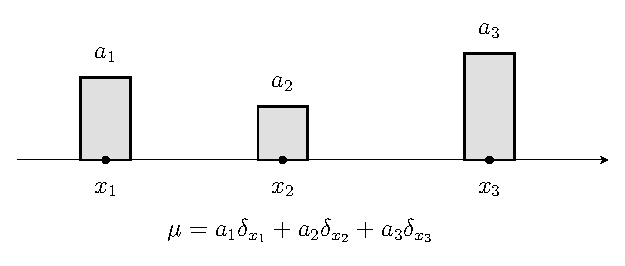
\includegraphics[width=0.76\textwidth]{miara-punktowa.pdf}
  \caption{Skończenie wiele punktów z przypisanymi wagami.}
  \label{fig:miara-punktowa}
\end{figure}

\section{Miara zewnętrzna Lebesgue'a}
\label{sec:miara-zewnetrzna-lebesgue}

\begin{definicja}[Miara zewnętrzna Lebesgue'a na prostej]
\label{def:miara-zewnetrzna-lebesgue}
Dla dowolnego $A\subseteq\R$ określamy
\begin{equation}
  \lambda^{\ast}(A)=\inf\left\{
    \sum_{n=1}^{\infty}|I_n|:
    A\subseteq\bigcup_{n=1}^{\infty}I_n,
    \ I_n\text{ są przedziałami}\right\}.
  \label{eq:miara-zewnetrzna-lebesgue}
\end{equation}
Symbol $|I_n|$ oznacza tu długość przedziału $I_n$.
Dla przedziału ograniczonego o końcach $a\leq b$ jest ona równa $b-a$,
niezależnie od uwzględnienia końców; przedziały nieograniczone mają
długość $+\infty$. Dopuszczamy przedziały jednopunktowe długości zero.
\end{definicja}

\begin{fakt}[Nieujemność i wartość na zbiorze pustym]
\label{fakt:zewnetrzna-zero}
Dla każdego $A\subseteq\R$ mamy $\lambda^{\ast}(A)\geq0$, a ponadto
$\lambda^{\ast}(\varnothing)=0$.
\end{fakt}

\begin{proof}
Każda suma długości przedziałów jest nieujemna, więc jej infimum
jest nieujemne. Zbiór pusty można pokryć ciągiem przedziałów
$I_n=[0,0]$; suma ich długości wynosi zero.
\end{proof}

\begin{fakt}[Monotoniczność miary zewnętrznej]
\label{fakt:zewnetrzna-monotonicznosc}
Jeżeli $A\subseteq B\subseteq\R$, to
$\lambda^{\ast}(A)\leq\lambda^{\ast}(B)$.
\end{fakt}

\begin{proof}
Każde pokrycie $B$ przedziałami pokrywa również $A$.
Zbiór dopuszczalnych sum długości dla $A$ zawiera więc zbiór
dopuszczalnych sum długości dla $B$. Przejście do infimów daje
żądaną nierówność.
\end{proof}

\begin{fakt}[Przeliczalna podaddytywność miary zewnętrznej]
\label{fakt:zewnetrzna-podaddytywnosc}
Dla dowolnych zbiorów $A_n\subseteq\R$ zachodzi
\begin{equation}
  \lambda^{\ast}\left(\bigcup_{n=1}^{\infty}A_n\right)
  \leq\sum_{n=1}^{\infty}\lambda^{\ast}(A_n).
  \label{eq:zewnetrzna-podaddytywnosc}
\end{equation}
\end{fakt}

\begin{proof}
Jeżeli suma po prawej stronie jest nieskończona, nierówność jest oczywista.
Załóżmy więc, że jest skończona, i ustalmy $\varepsilon>0$.
Dla każdego $n\geq1$ wybieramy pokrycie $A_n$ przedziałami
$I_1^{(n)},I_2^{(n)},\ldots$ takie, że
\[
  \sum_{k=1}^{\infty}|I_k^{(n)}|
  <\lambda^{\ast}(A_n)+\frac{\varepsilon}{2^n}.
\]
Możemy to zrobić z definicji infimum.
Rodzina $\{I_k^{(n)}:n,k\in\N\}$ jest przeliczalna i pokrywa
$\bigcup_{n=1}^{\infty}A_n$. Zatem
\begin{align*}
  \lambda^{\ast}\left(\bigcup_{n=1}^{\infty}A_n\right)
    &\leq\sum_{n=1}^{\infty}\sum_{k=1}^{\infty}|I_k^{(n)}|\\
    &\leq\sum_{n=1}^{\infty}
      \left(\lambda^{\ast}(A_n)+\frac{\varepsilon}{2^n}\right)\\
    &=\sum_{n=1}^{\infty}\lambda^{\ast}(A_n)+\varepsilon.
\end{align*}
Z dowolności $\varepsilon>0$ otrzymujemy
\eqref{eq:zewnetrzna-podaddytywnosc}.
\end{proof}
